Conditional on the six evaluation points the prediction of $Y(\theta)$ is illustrated in figure \ref{2cPred}. Furthermore, the probability that $Y(\theta)<0.30$ conditional on these points are shown in figure \ref{2bTheta}. 

From figure \ref{2cTheta}, one see that for $\theta = 0.36$ the probability of $Y(\theta)<0.30$ is maximal with probability/value $0.20$. One can also observe that $\theta = 0.25$ gives a probability of 0.16. Nevertheless, figure \ref{2cPred} illustrate that the variance is notably higher, with values .... and ... for respectively $\theta = 0.25$ and  $\theta = 0.36$

We will therefor suggest the scientist's to use $\theta = 0.36$. 

\begin{figure}
    \centering
    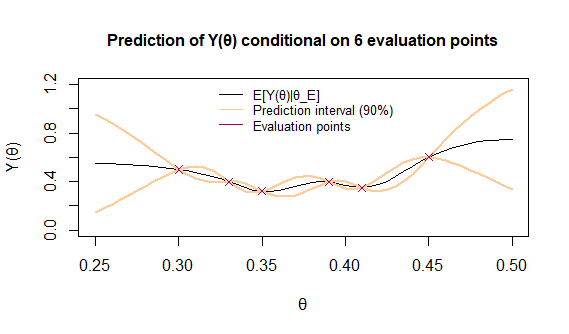
\includegraphics[width=100mm]{2cPred.png}
    \caption{Prediction of $Y(\theta)$ conditional on the six evaluation points  ($\theta$, $y(\theta)$): $(0.30,0.5)$, $(0.33, 0.40)$, $(0.35,0.32)$, $(0.39,0.40)$, $(0.41,0.35)$, and $(0.45,0.60)$. The graph includes a $90\%$ prediction interval. }
    \label{2cPred}
\end{figure}
\begin{figure}
    \centering
    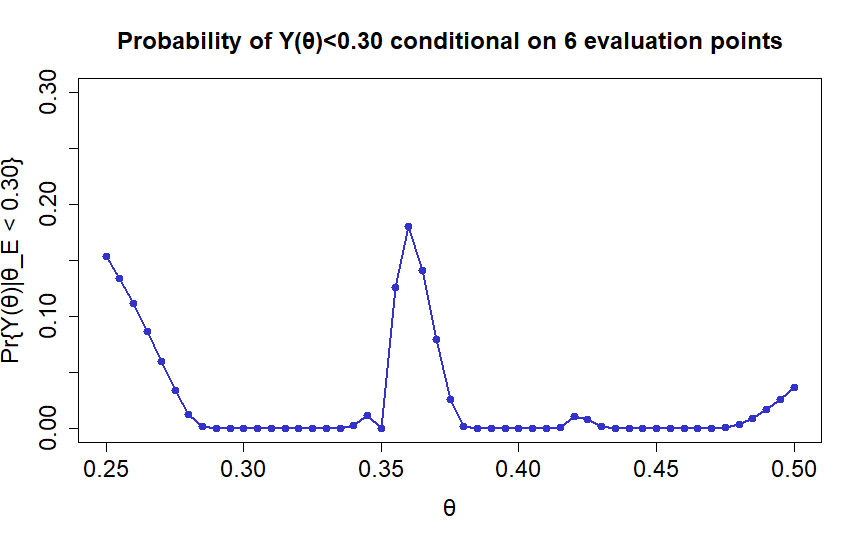
\includegraphics[width=100mm]{2ctheta.png}
    \caption{The probability of $Y(\theta)<0.30$ conditional on the six evaluation points ($\theta$, $y(\theta)$): $(0.30,0.5)$, $(0.33, 0.40)$, $(0.35,0.32)$, $(0.39,0.40)$, $(0.41,0.35)$, and $(0.45,0.60)$.}
    \label{2cTheta}
\end{figure}

Prediction of $Y(\theta)$ conditional on the six evaluation points given. The graph includes a $90\%$ prediction interval. 